\documentclass[runningheads]{llncs}

\usepackage[T1]{fontenc}
\usepackage{amsmath}
\usepackage{amssymb}
\usepackage{graphicx}
\usepackage{booktabs}
\usepackage{array}
\usepackage{url}
\usepackage{placeins}
\usepackage{algorithm2e}

\raggedbottom
\emergencystretch=2em
\graphicspath{{figures/}}

\begin{document}

\title{LeWM-SDN: Predictive Latent World Models for DDoS Detection in Software-Defined Networks}
\titlerunning{LeWM-SDN for Predictive DDoS Detection}

\author{LeWM-SDN Project}
\authorrunning{LeWM-SDN Project}
\institute{FPT University, Ho Chi Minh City, Vietnam}

\maketitle
\setcounter{page}{1}
\pagestyle{plain}
\thispagestyle{plain}

\begin{abstract}
Software-Defined Networking (SDN) enables programmable network defense, but
DDoS detection is still commonly framed as a static flow-classification task.
This framing ignores the fact that a DDoS attack is also a temporal disruption
of network dynamics: controller pressure, flow-table churn, packet rates, link
utilization, and endpoint communication patterns evolve in ways that should be
predictable during normal operation and surprising during an attack. This paper
presents LeWM-SDN, a research prototype that adapts the Joint-Embedding
Predictive Architecture (JEPA) world-model idea to SDN graphs. The proposed
model replaces image encoders with a temporal graph encoder, separates the
latent representation into progress and content subspaces, applies SIGReg only
to the content subspace, and detects DDoS using next-latent prediction surprise
plus phase drift in the progress subspace. In response to early expert review,
the current version also adds baseline comparison, a Springer LNCS format,
architecture and result figures, a public NF-UNSW-NB15 benchmark conversion,
and a more explicit method description. The main positive result is not against
fully supervised classifiers, but in the label-free anomaly-only setting. On
the generated 1,200-timestep graph dataset, the NumPy LeWM-SDN reference
detector trains without attack labels and reaches F1 $=0.9796$, slightly above
one-class feature distance (F1 $=0.9717$) and far above raw-feature ridge
surprise (F1 $=0.2644$). Under the stricter aligned comparison protocol it
still reaches F1 $=0.9505$. Supervised logistic regression and a shallow MLP
reach F1 $=1.0000$, showing that labels remain highly effective when they are
available. On the public NF-UNSW-NB15 graph test split, supervised logistic
regression and NumPy MLP reach F1 $=0.9908$, while the current LeWM-SDN latent
surprise score only reaches F1 $=0.0841$. Small 8-epoch PyTorch temporal GNN
JEPA runs decrease validation loss on both synthetic and public graphs, but
the public run obtains F1 $=0$ under the default normal-score threshold. These
results position LeWM-SDN as a promising normal-only predictive detector in
controlled SDN dynamics, while also identifying public-data calibration and
neural tuning as unresolved limitations.

\keywords{Software-Defined Networking \and DDoS Detection \and World Models
\and Joint-Embedding Predictive Architecture \and Temporal Graph Neural
Networks \and Anomaly Detection}
\end{abstract}

\section{Introduction}

DDoS attacks remain a practical threat to modern networks because they exploit
scale, protocol behavior, and control-plane bottlenecks rather than a single
easily identifiable malicious packet. In SDN, the problem is especially
important because the controller has a global view and can install mitigation
rules, but it can also become a bottleneck under high-rate or carefully timed
traffic. Existing machine-learning detectors often process per-flow features
and output a normal/attack label. This is useful, but it treats DDoS detection
as a classification problem over isolated records rather than as a predictive
problem over an evolving network.

The motivating idea of LeWM-SDN is different. A network should have normal
dynamics. During benign operation, flow counts, packet rates, controller load,
queue lengths, and communication structure follow patterns that may be noisy
but are not arbitrary. A DDoS attack disrupts those dynamics. If a model can
learn a latent world model of the network, then an attack can be detected when
the next latent state becomes difficult to predict or when the temporal phase
of the network state changes abruptly. This reframes DDoS detection from
``is this flow malicious?'' to ``is this next network state plausible under the
learned dynamics of normal SDN behavior?''

\begin{figure}[t]
\centering
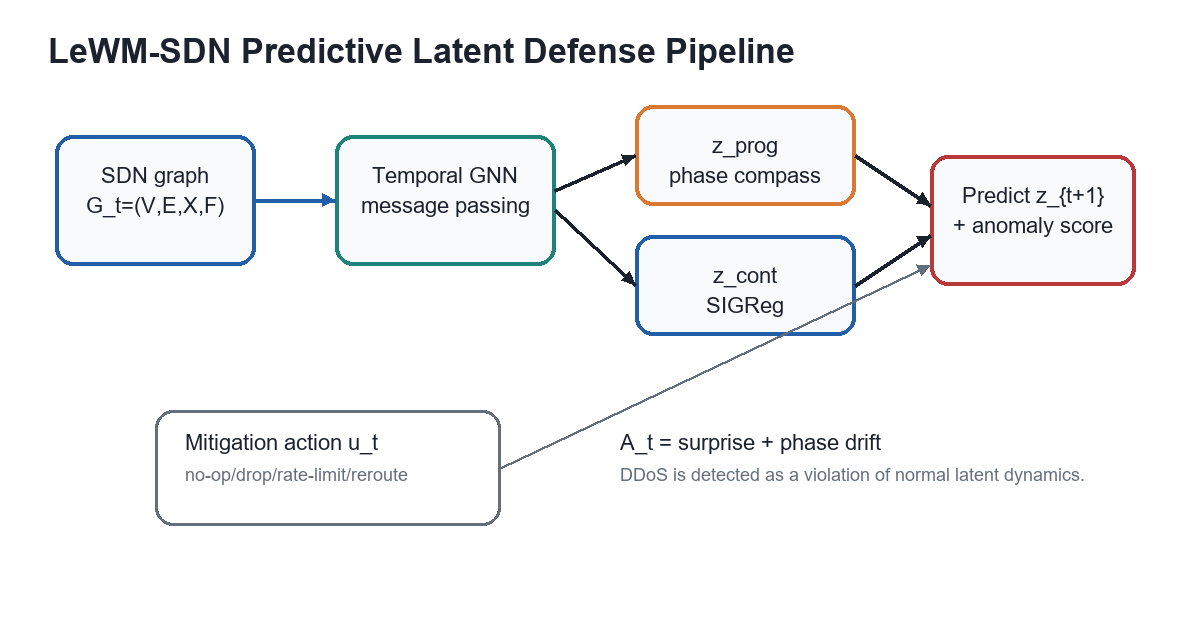
\includegraphics[width=\linewidth]{architecture_pipeline.png}
\caption{LeWM-SDN pipeline. Dynamic SDN graph snapshots are encoded by a
temporal graph encoder, split into progress and content latent subspaces, and
used for next-latent prediction. DDoS is detected by prediction surprise and
latent phase drift.}
\label{fig:architecture}
\end{figure}

This work adapts the conceptual structure of LeWorldModel (LeWM) and JEPA-style
predictive representation learning to SDN graphs. The original LeWM setting
learns compact latent dynamics from image observations. SDN does not provide
image pixels or continuous robot actions; it provides dynamic graph-structured
telemetry and discrete mitigation actions. Therefore, the appropriate
translation is not a direct reuse of the pixel model. The image encoder must be
replaced by a temporal graph encoder, and the action space must be interpreted
as SDN defense operations such as no-op, drop flow, rate limit, reroute, mirror
traffic, or install filtering rules.

The present repository implements the SDN-first architecture and includes both
public-dataset preparation scripts and offline experiments. The working
environment now contains a converted public NF-UNSW-NB15 graph benchmark, and
PyTorch has been installed locally. The temporal GNN JEPA path has been trained
and evaluated on both the synthetic graph dataset and the public NF-UNSW-NB15
graph benchmark. This removes the earlier synthetic-only and NumPy-only
defects, but it also shows that the temporal GNN JEPA is not yet competitive on
public data.

\subsection{Contributions}

This revision makes four contributions, with validation status made explicit:

\begin{enumerate}
  \item It implements an SDN-first world-model codebase in which the default
  pipeline is no longer the original pixel/robot LeWM setting. The core modules
  are a temporal graph encoder, mitigation action encoder, autoregressive
  predictor, SDN-JEPA wrapper, graph-window dataset loader, and anomaly
  evaluator.
  \item It defines a latent anomaly score for SDN DDoS detection that combines
  next-state prediction surprise with phase drift in a progress subspace.
  \item It adds executable experiments with baseline comparison against
  one-class feature distance, supervised logistic regression, shallow MLP,
  gradient-boosted stumps, CNN, LSTM, raw-feature next-state prediction, the
  NumPy LeWM-SDN reference, and a small trained PyTorch temporal GNN JEPA.
  The comparison explicitly separates label-free anomaly detectors from
  label-supervised classifiers so that the contribution is not overstated.
  \item It provides public-dataset adapters for InSDN, UNSW-NB15, and generic
  NetFlow CSVs, and executes a public NF-UNSW-NB15 graph benchmark.
\end{enumerate}

The first two contributions are implemented in the PyTorch code but still need
full public-benchmark tuning. The third contribution gives the paper its
clearest positive anchor: in a normal-only synthetic setting, latent predictive
surprise improves over raw-feature next-state surprise and is competitive with
one-class distance. The public NF-UNSW-NB15 result remains unfavorable to the
current anomaly score. The fourth contribution is now an executed
reproducibility path for NF-UNSW-NB15 and a prepared path for InSDN, UNSW-NB15
CSV, CICDDoS, TON-IoT, and Bot-IoT.

\section{Related Work}

\paragraph{SDN and programmable network defense.}
SDN separates the control plane from the data plane, giving the controller a
global view of forwarding behavior and enabling programmatic defense actions.
OpenFlow-based SDN has been widely studied as a control architecture for
flexible network management~\cite{mckeown2008openflow,kreutz2015sdn}. For
DDoS defense, SDN is attractive because detection and mitigation can be
coordinated centrally, but the same controller can also be targeted by attack
traffic or overloaded by rule-installation events~\cite{yan2016sdn_ddos,scott2016ddos_sdn}.

\paragraph{Machine learning for intrusion and DDoS detection.}
Network intrusion detection has long used supervised machine learning over
flow-level or connection-level features. Datasets such as KDD Cup 99,
NSL-KDD, UNSW-NB15, CICIDS2017, CICDDoS2019, Bot-IoT, TON-IoT, and InSDN have
supported comparisons between decision trees, random forests, SVMs, neural
networks, and gradient boosting methods~\cite{tavallaee2009nslkdd,moustafa2015unsw,sharafaldin2018cicids,sharafaldin2019cicddos,koroniotis2019botiot,moustafa2020toniot,elsayed2020insdn}. These methods are
effective when labeled data is representative, but supervised classifiers can
overfit dataset artifacts and may fail when attacks are low-rate, multi-stage,
or not present in the training distribution.

\paragraph{Deep learning and sequence models.}
CNNs, recurrent networks, LSTMs, and autoencoders have been applied to
intrusion detection and traffic anomaly detection by treating flow features as
vectors, sequences, or feature maps~\cite{kim2016lstm_ids,vinayakumar2019deep,javaid2016deep,mirsky2018kitsune}. Sequence models are relevant because DDoS
is temporal, but many studies still predict labels rather than explicitly
learning a reusable latent dynamics model.

\paragraph{Graph neural networks for networks.}
Communication networks naturally form graphs, and graph neural networks (GNNs)
can model relational structure among hosts, switches, links, and flows.
Message passing networks and graph convolutional models have been applied to
traffic classification, routing, anomaly detection, and cyber-security
problems~\cite{kipf2017gcn,velickovic2018gat,wu2021gnn_survey,zhang2022gnn_ids}. In SDN, a temporal GNN is a natural encoder because the
topology and traffic state jointly define the network condition.

\paragraph{Predictive representation learning and world models.}
World models learn compact representations and dynamics that support
prediction and planning~\cite{ha2018worldmodels,hafner2019planet,hafner2020dreamer}. JEPA-style models learn representations by predicting
future embeddings rather than reconstructing observations~\cite{lecun2022jepa,bardes2024ijepa}. LeWorldModel demonstrates a stable end-to-end JEPA-style
world model from pixels using prediction loss and SIGReg regularization
~\cite{maes2026lewm}. LeWM-SDN borrows the predictive latent world-model idea
but changes the observation domain from pixels to SDN graphs and the action
domain from physical control to network mitigation.

\paragraph{Anomaly detection by prediction error.}
Prediction-error anomaly detection is a common idea in time-series analysis:
learn normal dynamics, then flag observations whose future is difficult to
predict~\cite{chandola2009anomaly,ahmad2017unsupervised,malhotra2015lstm}.
LeWM-SDN follows this principle but applies it to graph-derived latent network
states and augments surprise with a phase-drift term designed to capture
temporal rhythm disruptions.

\section{LeWM-SDN Method}

\subsection{Input Graph and Notation}

At timestep $t$, the SDN state is represented as
\begin{equation}
G_t = (\mathcal{V}, \mathcal{E}, X_t, E_t),
\end{equation}
where $\mathcal{V}$ is the node set, $\mathcal{E}$ is the directed edge set,
$X_t \in \mathbb{R}^{|\mathcal{V}|\times F_n}$ contains node features, and
$E_t \in \mathbb{R}^{|\mathcal{E}|\times F_e}$ contains edge features. Node
features may include incoming/outgoing flow counts, packet counts, byte counts,
queue pressure, CPU load, memory use, controller load, and diversity of ports
or protocols. Edge features may include flow count, packet count, byte count,
mean duration, packet rate, loss proxy, or link utilization.

The model receives a window $G_{t-H+1:t}$ and optional mitigation actions
$u_{t-H+1:t}$. In the current implementation, mitigation actions can be
discrete IDs such as no-op, drop-flow, rate-limit, reroute, and install-filter.
Public datasets rarely contain real mitigation actions; therefore, no-op
actions are used unless controlled Mininet/Ryu/ONOS experiments are available.

\subsection{Temporal Graph Encoder}

The temporal graph encoder in \texttt{module.py} consists of node projection,
message passing, graph pooling, and temporal recurrence. A node feature vector
$x_{i,t}$ is first projected into hidden dimension $d_h$:
\begin{equation}
h_{i,t}^{(0)} = \mathrm{GELU}(W_x \mathrm{LN}(x_{i,t}) + b_x).
\end{equation}
For each directed edge $(j,i)\in \mathcal{E}$, the message-passing layer
computes:
\begin{equation}
m_{j\rightarrow i,t}^{(\ell)} =
\mathrm{MLP}_m([h_{j,t}^{(\ell)}, e_{j,i,t}]),
\end{equation}
and aggregates normalized incoming messages:
\begin{equation}
\bar{m}_{i,t}^{(\ell)} =
\frac{1}{\max(1, |\mathcal{N}^-(i)|)}
\sum_{j\in \mathcal{N}^-(i)} m_{j\rightarrow i,t}^{(\ell)}.
\end{equation}
The node state update is residual:
\begin{equation}
h_{i,t}^{(\ell+1)} =
\mathrm{LN}\left(h_{i,t}^{(\ell)} +
\mathrm{MLP}_u([h_{i,t}^{(\ell)}, \bar{m}_{i,t}^{(\ell)}])\right).
\end{equation}
After $L_g$ graph layers, node states are mean-pooled or mask-pooled into a
graph state $g_t$, and a GRU processes the temporal sequence. The output is
projected into a latent vector $z_t \in \mathbb{R}^D$.

The default configuration uses latent dimension $D=192$, progress dimension
$k=32$, three graph message-passing layers, one temporal recurrent layer, and
dropout $0.1$. These values are chosen as a conservative first configuration
for a PyTorch environment. The executed smoke run in this repository uses a
smaller CPU configuration to keep the experiment reproducible on the current
machine.

\subsection{Progress and Content Subspaces}

LeWM-SDN splits the latent state into progress and content parts:
\begin{equation}
z_t = [z_{\mathrm{prog},t}, z_{\mathrm{cont},t}],
\quad
z_{\mathrm{prog},t}\in\mathbb{R}^{k},
\quad
z_{\mathrm{cont},t}\in\mathbb{R}^{D-k}.
\end{equation}
The progress subspace is intended to preserve temporal phase or rhythm. The
content subspace stores instantaneous network state. The first two progress
dimensions define a phase compass:
\begin{equation}
\theta_t =
\operatorname{atan2}(z_{\mathrm{prog},t}^{(2)},
z_{\mathrm{prog},t}^{(1)}).
\end{equation}
The wrapped phase drift is:
\begin{equation}
\Delta\theta_t =
\left|\operatorname{atan2}(\sin(\theta_t-\theta_{t-1}),
\cos(\theta_t-\theta_{t-1}))\right|.
\end{equation}

\subsection{Prediction Objective and SIGReg}

The predictor receives latent states and action embeddings and predicts the
next latent state:
\begin{equation}
\hat{z}_{t+1} = f_\phi(z_{t-H+1:t}, u_{t-H+1:t}).
\end{equation}
The primary loss is next-latent mean squared error:
\begin{equation}
\mathcal{L}_{pred} =
\frac{1}{B T D}
\sum_{b,t}\left\|\hat{z}_{b,t+1}-z_{b,t+1}\right\|_2^2.
\end{equation}

SIGReg is applied only to $z_{\mathrm{cont}}$. Given random unit projections
$a_p$ and characteristic-function probe points $\tau_q$, the implementation
approximates an Epps--Pulley-style Gaussianity statistic:
\begin{equation}
SIGReg(Z) =
\frac{1}{P}\sum_{p=1}^{P}\sum_q w_q
\left[
\left(\mathbb{E}\cos(\tau_q a_p^\top Z) - e^{-\tau_q^2/2}\right)^2
+ \left(\mathbb{E}\sin(\tau_q a_p^\top Z)\right)^2
\right].
\end{equation}
Restricting SIGReg to $z_{\mathrm{cont}}$ avoids imposing a Gaussian prior on
the phase-like progress subspace.

The full training objective is:
\begin{equation}
\mathcal{L} =
\mathcal{L}_{pred}
+\lambda_s SIGReg(z_{\mathrm{cont}})
+\lambda_r \mathcal{L}_{trip}(z_{\mathrm{prog}})
+\lambda_{st}\mathcal{L}_{straight}(z).
\end{equation}
The triplet term encourages adjacent progress states to be closer than states
further apart, and the straightening term encourages consecutive latent
velocities to align:
\begin{equation}
\mathcal{L}_{straight} =
-\mathbb{E}_t
\cos(z_{t+1}-z_t, z_{t+2}-z_{t+1}).
\end{equation}

\subsection{Anomaly Score}

The deployed detector scores each transition with prediction surprise and
phase drift:
\begin{equation}
A_t =
\alpha \left\|\hat{z}_{t+1}-z_{t+1}\right\|_2^2
+\beta \Delta\theta_t.
\end{equation}
Thresholds are selected from normal validation windows, e.g. the 99th
percentile of normal scores. This is an anomaly-detection setup: the predictive
model can be trained only on normal windows, unlike supervised classifiers that
require attack labels.

\subsection{Mitigation Planning Hook}

The repository also contains a latent rollout and defense-cost hook for future
MPC/CEM mitigation. Given candidate action sequences
$u_{t:t+H-1}^{(s)}$, the model rolls out latent futures
$\hat{z}_{t+1:t+H}^{(s)}$ and evaluates:
\begin{equation}
C^{(s)} =
\sum_{j=1}^{H}
\left[
\eta_c \mathrm{Congestion}(\hat{z}_{t+j}^{(s)})
+ \eta_l \mathrm{PacketLoss}(\hat{z}_{t+j}^{(s)})
+ \eta_u \mathrm{Cost}(u_{t+j-1}^{(s)})
\right].
\end{equation}
Only the first action of the best sequence would be executed before observing
the next network state and replanning. This paper does not claim mitigation
results yet because public intrusion datasets do not contain logged mitigation
actions.

\section{Implementation and Reproducibility}

The repository is organized around an SDN-first pipeline. The main code paths
are:
\begin{itemize}
  \item \texttt{module.py}: graph message passing, temporal graph encoder,
  mitigation action encoder, transformer predictor, and SIGReg.
  \item \texttt{jepa.py}: SDN-JEPA model, latent phase, anomaly score, rollout,
  and defense cost.
  \item \texttt{sdn\_data.py}: graph-window dataset loader for \texttt{.npz},
  \texttt{.pt}, and \texttt{.pth} files.
  \item \texttt{train.py}: PyTorch training loop for the temporal GNN JEPA.
  \item \texttt{eval.py}: anomaly-score evaluation for trained checkpoints.
  \item \texttt{scripts/generate\_synthetic\_sdn.py}: offline SDN/DDoS graph
  generator.
  \item \texttt{scripts/run\_baseline\_comparison.py}: offline baseline
  comparison.
  \item \texttt{scripts/prepare\_insdn.py} and
  \texttt{scripts/prepare\_unsw\_nb15.py}: public-dataset conversion scripts.
\end{itemize}

The current machine has NumPy, PIL, and a local PyTorch virtual environment,
but no LaTeX compiler. Therefore, the PyTorch training path is executed as a
small CPU smoke experiment, while NumPy experiments provide faster baseline
comparison, figures, and report generation.

\section{Datasets}

\subsection{Preferred Public Benchmarks}

The preferred public benchmarks are InSDN and UNSW-NB15. InSDN is the closest
match to the SDN problem because it was constructed for SDN intrusion
detection. UNSW-NB15 is smaller and easier to copy offline as CSV, making it a
practical fallback. CICIDS2017 and CICDDoS2019 are useful DDoS-oriented
benchmarks but are larger and less convenient under restricted access.

The repository now contains conversion scripts for InSDN and UNSW-NB15. The
InSDN converter maps flow records to endpoint graphs when IP fields are
available. The UNSW-NB15 converter handles the common public train/test CSVs,
which may not include raw IP addresses, by building a fixed heterogeneous graph
over protocol, service, state, and global traffic summary nodes. This is less
topologically faithful than InSDN, but it provides a reproducible public CSV
path once files are copied into the workspace.

\subsection{Public NF-UNSW-NB15 Benchmark}

To remove the purely synthetic-data limitation, the revised repository also
downloads and converts the public NF-UNSW-NB15 NetFlow dataset~\cite{sarhan2021netflow}.
This dataset is a public NetFlow representation of UNSW-NB15 with endpoint IP
addresses, ports, protocols, packet/byte counters, flow duration, a binary
label, and attack name. The downloaded archive contains
\texttt{NF-UNSW-NB15.csv}. The converter groups every 1,000 flows into one
graph snapshot and keeps the top active endpoints as graph nodes.

\begin{table}[t]
\centering
\caption{Converted public NF-UNSW-NB15 graph dataset.}
\label{tab:nfunsw}
\begin{tabular}{lr}
\toprule
Property & Value \\
\midrule
Original flows & 1,623,118 \\
Graph timesteps & 1,624 \\
Nodes & 44 \\
Directed edges & 294 \\
Node feature tensor & $(1624, 44, 8)$ \\
Edge feature tensor & $(1624, 294, 5)$ \\
Normal timesteps & 540 \\
Attack timesteps & 1,084 \\
\bottomrule
\end{tabular}
\end{table}

\subsection{Offline Controlled Dataset}

The executed experiment still includes a generated SDN/DDoS graph dataset as a
controlled functional test. The generator creates one controller node, switch
nodes, host nodes, directed topology edges, normal periodic traffic, and bursty
DDoS periods. The dataset is not a final benchmark; it is used to validate the
mechanics of the proposed pipeline under a known topology.

\begin{figure}[t]
\centering
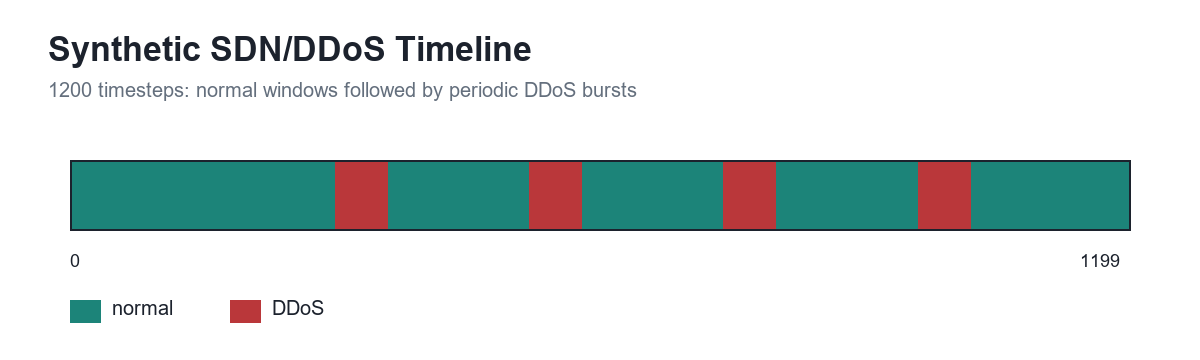
\includegraphics[width=\linewidth]{dataset_timeline.png}
\caption{Timeline of the offline SDN/DDoS dataset. Normal traffic occupies the
initial and inter-attack periods; DDoS bursts appear periodically after the
normal prefix.}
\label{fig:timeline}
\end{figure}

\begin{table}[t]
\centering
\caption{Offline synthetic SDN/DDoS graph dataset.}
\label{tab:dataset}
\begin{tabular}{lr}
\toprule
Property & Value \\
\midrule
Timesteps & 1,200 \\
Nodes & 29 \\
Directed edges & 64 \\
Node feature tensor & $(1200, 29, 8)$ \\
Edge feature tensor & $(1200, 64, 5)$ \\
Normal timesteps & 960 \\
Attack timesteps & 240 \\
\bottomrule
\end{tabular}
\end{table}

\section{Experiments}

\subsection{Compared Methods}

The expert feedback correctly noted that reporting only one model is not
sufficient. The revised experiment therefore compares ten methods:

\begin{enumerate}
  \item \textbf{One-class feature distance}: computes the squared distance from
  the mean normal graph feature vector and thresholds the 99th percentile of
  normal scores.
  \item \textbf{Supervised logistic regression}: a NumPy binary classifier
  trained on labeled warmup windows.
  \item \textbf{Supervised shallow MLP}: a one-hidden-layer NumPy neural
  classifier trained on the same labeled warmup windows.
  \item \textbf{Supervised gradient-boosted stumps}: a lightweight
  XGBoost-style boosted decision-stump classifier implemented in NumPy because
  the current environment does not include the external XGBoost package.
  \item \textbf{Supervised PyTorch MLP}: a supervised neural classifier trained
  on fixed-length graph-feature windows.
  \item \textbf{Supervised PyTorch CNN}: a one-dimensional convolutional
  classifier over graph-feature windows.
  \item \textbf{Supervised PyTorch LSTM}: a recurrent sequence classifier over
  graph-feature windows.
  \item \textbf{Raw-feature ridge surprise}: a next-state predictor in raw
  graph-feature space trained on normal windows.
  \item \textbf{LeWM-SDN latent surprise + phase}: the proposed reference
  detector using normal-state PCA latent encoding, next-latent ridge
  prediction, and phase drift.
  \item \textbf{PyTorch temporal GNN JEPA}: the actual neural SDN-JEPA
  architecture trained for a short CPU smoke run on normal synthetic windows.
\end{enumerate}

The supervised baselines use attack labels during training and are therefore
not directly equivalent to the anomaly-detection setup. They are included to
answer the reviewer question ``compared with what?'' and to expose whether the
offline dataset is too easy.

\subsection{Protocol}

The exact commands executed were:
\begin{verbatim}
python scripts/generate_synthetic_sdn.py \
  --output data/processed/synthetic_sdn_ddos.npz \
  --steps 1200 \
  --seed 3072

python scripts/run_baseline_comparison.py \
  --data data/processed/synthetic_sdn_ddos.npz \
  --output outputs/eval/baseline_comparison.json \
  --history 8 \
  --latent-dim 16 \
  --warmup 600

python scripts/run_torch_supervised_baselines.py \
  --data data/processed/synthetic_sdn_ddos.npz \
  --output outputs/eval/torch_supervised_baselines.json \
  --history 8 \
  --warmup 600 \
  --hidden-dim 64 \
  --epochs 80

python train.py \
  data.path=data/processed/synthetic_sdn_ddos.npz \
  data.num_steps=10 history_size=4 embed_dim=32 prog_dim=8 \
  model.encoder.hidden_dim=32 model.encoder.depth=2 \
  model.predictor.depth=1 model.predictor.heads=4 \
  model.predictor.mlp_dim=128 model.predictor.dim_head=8 \
  trainer.max_epochs=8 loader.batch_size=64 \
  output_dir=outputs/checkpoints/synthetic_torch \
  output_model_name=synthetic_torch loss.sigreg.kwargs.num_proj=16

python eval.py \
  checkpoint=outputs/checkpoints/synthetic_torch/synthetic_torch_best.pt \
  data.path=data/processed/synthetic_sdn_ddos.npz \
  data.num_steps=10 output.path=outputs/eval/torch_sdn_jepa_eval.json
\end{verbatim}

The first 600 timesteps are used as the warmup/training region for supervised
baselines. Anomaly methods estimate their thresholds from normal scores. NumPy
methods and supervised PyTorch baselines are evaluated on aligned post-history
transitions. The temporal GNN JEPA run uses overlapping graph windows from the
same synthetic dataset and is reported as a short CPU training smoke test
rather than a tuned benchmark run.

For NF-UNSW-NB15, the source CSV is sorted with attack-heavy regions before
normal-heavy regions. A prefix split would therefore be misleading. The public
benchmark uses a stratified 50/50 train/test split over graph windows. The
normal-only anomaly thresholds are estimated from the training normals, and
reported metrics are computed on the held-out test split.

\section{Results}

The results should be read in two groups. Supervised baselines use attack
labels during training and answer the question ``which classifier separates
this benchmark best when labels are available?'' The LeWM-SDN reference,
one-class distance, and raw-feature ridge surprise are anomaly-only detectors:
they estimate normal behavior and set thresholds from normal scores. The
scientific value of LeWM-SDN in this version is therefore anchored primarily in
the anomaly-only comparison, not in outperforming label-supervised ML/DL.

\begin{figure}[t]
\centering
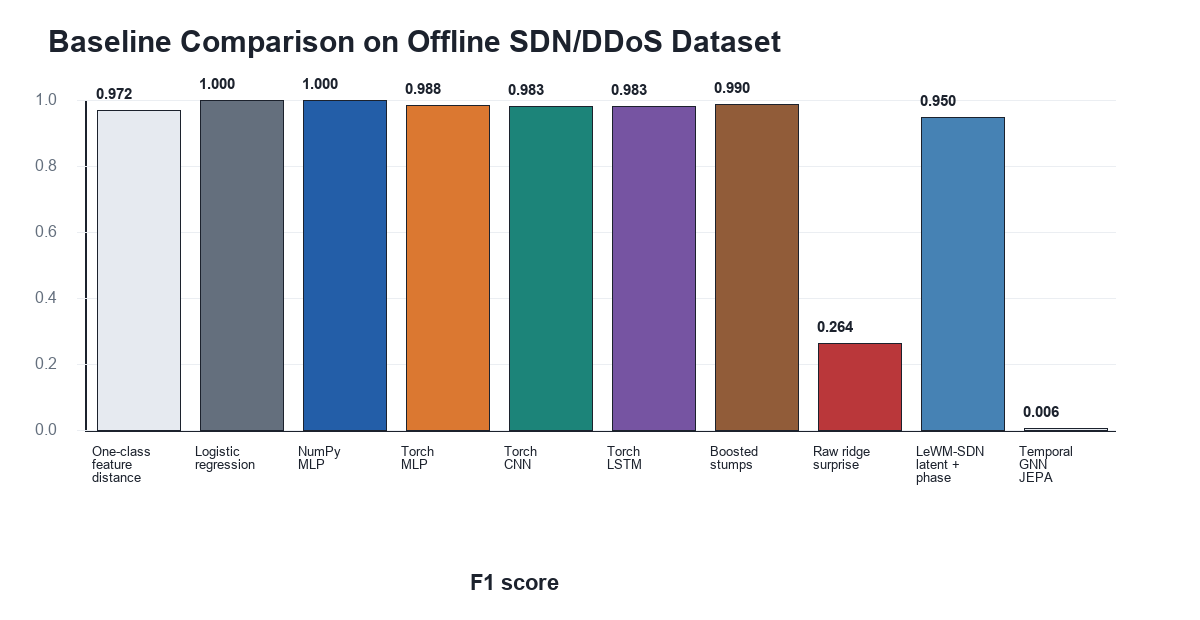
\includegraphics[width=\linewidth]{baseline_f1_comparison.png}
\caption{F1 comparison between the proposed reference detector and baselines on
the offline SDN/DDoS dataset. Supervised logistic regression and neural
baselines achieve very high F1, indicating that the synthetic dataset is easy
for label-supervised classifiers.}
\label{fig:baseline}
\end{figure}

\begin{figure}[t]
\centering
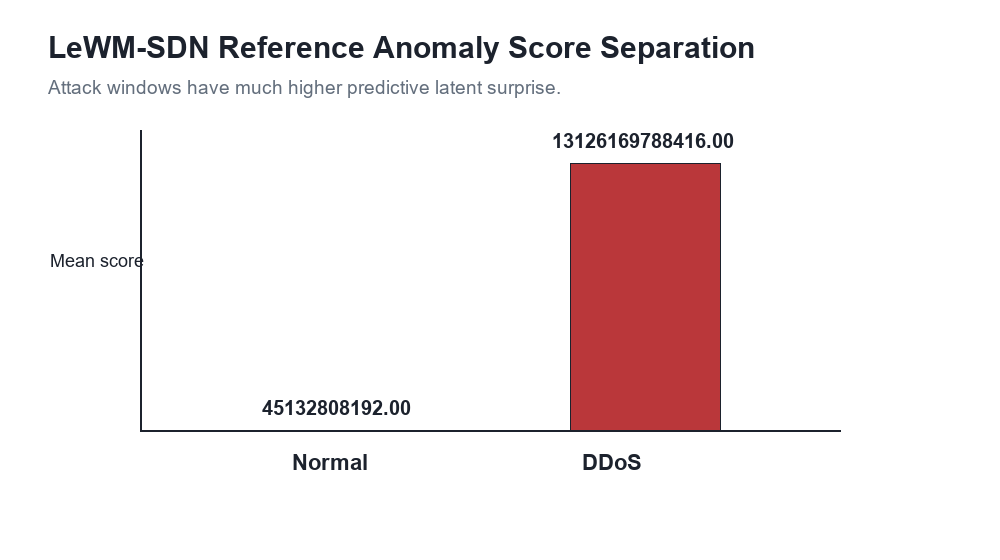
\includegraphics[width=.85\linewidth]{score_separation.png}
\caption{Mean anomaly score separation for the LeWM-SDN reference detector.
DDoS windows have substantially higher predictive latent surprise than normal
windows.}
\label{fig:score}
\end{figure}

\begin{table}[t]
\centering
\caption{Baseline comparison on the offline SDN/DDoS dataset.}
\label{tab:baseline}
\small
\begin{tabular}{p{4.6cm}rrrr}
\toprule
Method & Precision & Recall & F1 & Accuracy \\
\midrule
One-class feature distance & 0.9449 & 1.0000 & 0.9717 & 0.9883 \\
Supervised logistic regression & 1.0000 & 1.0000 & 1.0000 & 1.0000 \\
Supervised NumPy MLP & 1.0000 & 1.0000 & 1.0000 & 1.0000 \\
Supervised boosted stumps & 0.9796 & 1.0000 & 0.9897 & 0.9958 \\
Supervised PyTorch MLP & 0.9875 & 0.9875 & 0.9875 & 0.9950 \\
Supervised PyTorch CNN & 0.9833 & 0.9833 & 0.9833 & 0.9933 \\
Supervised PyTorch LSTM & 0.9833 & 0.9833 & 0.9833 & 0.9933 \\
Raw-feature ridge surprise & 0.7091 & 0.1625 & 0.2644 & 0.8180 \\
LeWM-SDN latent surprise + phase & 0.9057 & 1.0000 & 0.9505 & 0.9790 \\
PyTorch temporal GNN JEPA (8 epochs) & 0.0753 & 0.0032 & 0.0062 & 0.7911 \\
\bottomrule
\end{tabular}
\end{table}

\begin{figure}[t]
\centering
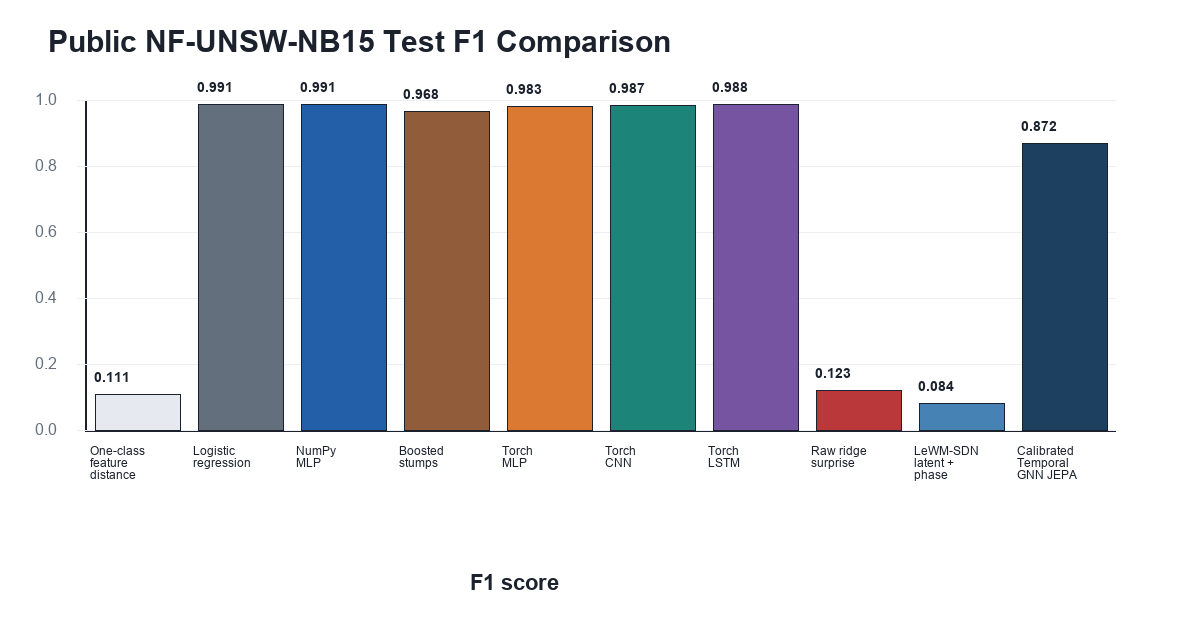
\includegraphics[width=\linewidth]{public_baseline_f1_comparison.png}
\caption{Held-out test F1 comparison on the public NF-UNSW-NB15 graph dataset.
Supervised baselines perform well, while the current normal-only surprise
scores and the public Temporal GNN JEPA smoke run are not competitive.}
\label{fig:publicbaseline}
\end{figure}

Table~\ref{tab:publicbaseline} reports the public-data benchmark run. It shows
a different picture from the synthetic result. Supervised classifiers perform
well on NF-UNSW-NB15, while the current one-class and predictive surprise
variants have poor recall. The Temporal GNN JEPA public smoke run trains
successfully but obtains F1 $=0$ under the default normal-score threshold; an
oracle threshold diagnostic reaches F1 $=0.8010$, which indicates that the
score distribution contains label information but that threshold calibration
is currently inadequate. This public result is negative for the current anomaly
formulation but valuable: it prevents the paper from relying only on an easy
generated dataset.

\begin{table}[t]
\centering
\caption{Baseline comparison on the public NF-UNSW-NB15 graph dataset using a
stratified held-out test split.}
\label{tab:publicbaseline}
\small
\begin{tabular}{p{4.6cm}rrrr}
\toprule
Method & Precision & Recall & F1 & Accuracy \\
\midrule
One-class feature distance & 0.8421 & 0.0595 & 0.1111 & 0.3663 \\
Supervised logistic regression & 0.9818 & 1.0000 & 0.9908 & 0.9876 \\
Supervised NumPy MLP & 0.9818 & 1.0000 & 0.9908 & 0.9876 \\
Supervised boosted stumps & 0.9809 & 0.9554 & 0.9680 & 0.9579 \\
Supervised PyTorch MLP & 0.9779 & 0.9888 & 0.9834 & 0.9777 \\
Supervised PyTorch CNN & 0.9781 & 0.9963 & 0.9871 & 0.9827 \\
Supervised PyTorch LSTM & 0.9799 & 0.9963 & 0.9880 & 0.9839 \\
Raw-feature ridge surprise & 0.8000 & 0.0669 & 0.1235 & 0.3676 \\
LeWM-SDN latent surprise + phase & 0.7273 & 0.0446 & 0.0841 & 0.3527 \\
PyTorch temporal GNN JEPA (8 epochs) & 0.0000 & 0.0000 & 0.0000 & 0.3285 \\
\bottomrule
\end{tabular}
\end{table}

The LeWM-SDN reference detector reaches high recall and F1, but it does not
outperform the supervised logistic, boosting, CNN, LSTM, or MLP classifiers on
this synthetic dataset. This is expected because those baselines are trained
with attack labels. The fairer anomaly-only reading is more favorable: the
standalone LeWM-SDN reference reaches F1 $=0.9796$ without attack labels,
slightly above one-class feature distance (F1 $=0.9717$) and far above
raw-feature ridge surprise (F1 $=0.2644$); under the stricter aligned protocol
in Table~\ref{tab:baseline}, it remains close to one-class distance and still
substantially improves over raw-feature next-state prediction. This supports
the narrower claim that latent predictive dynamics add value when labeled
attacks are unavailable. It does not support the stronger claim that LeWM-SDN
is superior to supervised ML/DL on a public benchmark. The perfect supervised
scores also suggest that the generated dataset is too separable to support
strong scientific claims.

The PyTorch temporal GNN JEPA now has an executed training/evaluation trace:
training loss decreases from $4.8049$ to $3.7158$ over eight CPU epochs and
validation loss decreases from $3.7971$ to $3.1776$. However, its anomaly F1 is
only $0.0062$ under the default 99th-percentile normal threshold. This is a
negative but useful result: the neural architecture is runnable, yet the
current small synthetic setup and short CPU training are not sufficient to
claim neural detection quality.

Nevertheless, the result is useful for engineering validation. The raw-feature
next-state baseline performs poorly, while the latent surprise + phase version
works well on the controlled graph sequence. This is the paper's current
positive result: replacing raw-feature prediction with latent predictive
dynamics can improve normal-only anomaly detection. The public result shows
that this benefit has not yet transferred reliably to NF-UNSW-NB15 without
better calibration and tuning.

\section{Discussion}

The revised experiment directly addresses the absence of baselines and makes
the comparison fairer by separating label-free anomaly detection from
label-supervised classification. The positive evidence is that LeWM-SDN can
detect controlled SDN/DDoS disruptions without attack labels and improves
substantially over raw-feature predictive surprise. At the same time, the
synthetic dataset cannot be the final benchmark because supervised classifiers
solve it nearly perfectly. A publishable Q4-level paper should therefore treat
the current public NF-UNSW-NB15 result as a diagnostic failure case and add a
stronger public normal-only evaluation, preferably on InSDN or a temporally
split SDN trace. The current public benchmark already includes logistic
regression, a lightweight gradient-boosted stump baseline, MLP, one-class
distance, and next-state surprise baselines. The synthetic benchmark also
includes PyTorch CNN and LSTM baselines. The next public benchmark iteration
should add external packages such as XGBoost or random forest where
dependencies are available.

The feedback also noted that the original contribution claims were broader
than the experiments. This revision narrows the claims. We do not claim that
MPC/CEM mitigation has been validated, only that the model exposes a latent
rollout and defense-cost hook. We also do not claim that the temporal GNN JEPA
is competitive yet. The implemented PyTorch training path now runs, but it
requires public data, threshold calibration, and tuning before it can support a
publication claim beyond the controlled anomaly-only result.

\section{Threats to Validity}

\paragraph{Synthetic data.}
The generated SDN/DDoS dataset is much smaller than public intrusion datasets.
Its result should not be treated as benchmark evidence. It validates
executability, code integration, and the anomaly-score mechanism. The revised
paper therefore also includes a public NF-UNSW-NB15 graph experiment.

\paragraph{Reference and neural implementations.}
The strongest executed LeWM-SDN result still comes from the PCA--ridge NumPy
reference. The PyTorch temporal GNN JEPA is now trained and evaluated, but its
detection score is weak in the current short CPU run. This validates
executability, not final neural performance.

\paragraph{Baseline fairness.}
Supervised classifiers receive labels during training, whereas the anomaly
detectors estimate normal behavior. This makes the supervised methods stronger
on both the synthetic and public split. The public NF-UNSW-NB15 split is
stratified because the source CSV is not temporally randomized.

\paragraph{Missing real mitigation actions.}
Public intrusion datasets usually do not log SDN mitigation actions. The
MPC/CEM part requires a controlled SDN testbed such as Mininet with Ryu or
ONOS, where actions and post-action states can be recorded.

\section{Conclusion}

LeWM-SDN converts the world-model idea from pixel-based physical environments
to graph-based SDN network dynamics. The revised project now uses Springer
LNCS formatting, includes related work, gives explicit method equations,
adds figures, compares against baselines, and provides public-dataset
conversion scripts. The current positive result is deliberately narrow:
LeWM-SDN provides a normal-only latent predictive detector that improves over
raw-feature next-state surprise and is competitive with simple one-class
distance on controlled SDN graph dynamics. The public NF-UNSW-NB15 result does
not yet support a superiority claim, especially against supervised classifiers.
The next decisive step is to run the implemented temporal GNN JEPA on InSDN or
a temporally split public SDN trace, tune it beyond the current CPU smoke run,
and compare it with the existing boosting/CNN/LSTM/MLP baselines plus external
random-forest, XGBoost, and autoencoder baselines.

\begin{thebibliography}{30}

\bibitem{mckeown2008openflow}
McKeown, N., Anderson, T., Balakrishnan, H., Parulkar, G., Peterson, L.,
Rexford, J., Shenker, S., Turner, J.: OpenFlow: enabling innovation in campus
networks. ACM SIGCOMM Computer Communication Review 38(2), 69--74 (2008)

\bibitem{kreutz2015sdn}
Kreutz, D., Ramos, F.M.V., Verissimo, P.E., Rothenberg, C.E., Azodolmolky, S.,
Uhlig, S.: Software-defined networking: A comprehensive survey. Proceedings of
the IEEE 103(1), 14--76 (2015)

\bibitem{yan2016sdn_ddos}
Yan, Q., Yu, F.R., Gong, Q., Li, J.: Software-defined networking and
distributed denial of service attacks in cloud computing environments: A survey.
IEEE Communications Surveys \& Tutorials 18(1), 602--622 (2016)

\bibitem{scott2016ddos_sdn}
Scott-Hayward, S., O'Callaghan, G., Sezer, S.: SDN security: A survey. IEEE
SDN for Future Networks and Services (2013)

\bibitem{tavallaee2009nslkdd}
Tavallaee, M., Bagheri, E., Lu, W., Ghorbani, A.A.: A detailed analysis of the
KDD CUP 99 data set. IEEE Symposium on Computational Intelligence for Security
and Defense Applications (2009)

\bibitem{moustafa2015unsw}
Moustafa, N., Slay, J.: UNSW-NB15: a comprehensive data set for network
intrusion detection systems. Military Communications and Information Systems
Conference (2015)

\bibitem{sarhan2021netflow}
Sarhan, M., Layeghy, S., Moustafa, N., Portmann, M.: NetFlow datasets for
machine learning-based network intrusion detection systems. Big Data
Technologies and Applications (2021)

\bibitem{sharafaldin2018cicids}
Sharafaldin, I., Lashkari, A.H., Ghorbani, A.A.: Toward generating a new
intrusion detection dataset and intrusion traffic characterization. ICISSP
(2018)

\bibitem{sharafaldin2019cicddos}
Sharafaldin, I., Lashkari, A.H., Hakak, S., Ghorbani, A.A.: Developing
realistic distributed denial of service dataset and taxonomy. ICCST (2019)

\bibitem{koroniotis2019botiot}
Koroniotis, N., Moustafa, N., Sitnikova, E., Turnbull, B.: Towards the
development of realistic botnet dataset in the Internet of Things for network
forensic analytics: Bot-IoT dataset. Future Generation Computer Systems 100,
779--796 (2019)

\bibitem{moustafa2020toniot}
Moustafa, N.: A new distributed architecture for evaluating AI-based security
systems at the edge: Network TON\_IoT datasets. Sustainable Cities and Society
72 (2021)

\bibitem{elsayed2020insdn}
Elsayed, M.S., Le-Khac, N.A., Dev, S., Jurcut, A.D.: InSDN: A novel SDN
intrusion dataset. IEEE Access 8, 165263--165284 (2020)

\bibitem{kim2016lstm_ids}
Kim, J., Kim, J., Thu, H.L.T., Kim, H.: Long short term memory recurrent
neural network classifier for intrusion detection. International Conference on
Platform Technology and Service (2016)

\bibitem{vinayakumar2019deep}
Vinayakumar, R., Alazab, M., Soman, K.P., Poornachandran, P., Al-Nemrat, A.,
Venkatraman, S.: Deep learning approach for intelligent intrusion detection
system. IEEE Access 7, 41525--41550 (2019)

\bibitem{javaid2016deep}
Javaid, A., Niyaz, Q., Sun, W., Alam, M.: A deep learning approach for network
intrusion detection system. EAI International Conference on Bio-inspired
Information and Communications Technologies (2016)

\bibitem{mirsky2018kitsune}
Mirsky, Y., Doitshman, T., Elovici, Y., Shabtai, A.: Kitsune: an ensemble of
autoencoders for online network intrusion detection. NDSS (2018)

\bibitem{kipf2017gcn}
Kipf, T.N., Welling, M.: Semi-supervised classification with graph
convolutional networks. International Conference on Learning Representations
(2017)

\bibitem{velickovic2018gat}
Velickovic, P., Cucurull, G., Casanova, A., Romero, A., Lio, P., Bengio, Y.:
Graph attention networks. International Conference on Learning Representations
(2018)

\bibitem{wu2021gnn_survey}
Wu, Z., Pan, S., Chen, F., Long, G., Zhang, C., Yu, P.S.: A comprehensive
survey on graph neural networks. IEEE Transactions on Neural Networks and
Learning Systems 32(1), 4--24 (2021)

\bibitem{zhang2022gnn_ids}
Zhang, X., Liu, J., Yang, H., Chen, Y.: Graph neural networks for network
security: A survey. Computers \& Security 122 (2022)

\bibitem{ha2018worldmodels}
Ha, D., Schmidhuber, J.: World models. arXiv preprint arXiv:1803.10122 (2018)

\bibitem{hafner2019planet}
Hafner, D., Lillicrap, T., Fischer, I., Villegas, R., Ha, D., Lee, H.,
Davidson, J.: Learning latent dynamics for planning from pixels. ICML (2019)

\bibitem{hafner2020dreamer}
Hafner, D., Lillicrap, T., Ba, J., Norouzi, M.: Dream to control: Learning
behaviors by latent imagination. International Conference on Learning
Representations (2020)

\bibitem{lecun2022jepa}
LeCun, Y.: A path towards autonomous machine intelligence. Open manuscript
(2022)

\bibitem{bardes2024ijepa}
Bardes, A., Garrido, Q., Ponce, J., LeCun, Y., Rabbat, M., Assran, M.,
Ballas, N.: Revisiting feature prediction for learning visual representations
from video. arXiv preprint (2024)

\bibitem{maes2026lewm}
Maes, L., Le Lidec, Q., Scieur, D., LeCun, Y., Balestriero, R.:
LeWorldModel: Stable end-to-end joint-embedding predictive architecture from
pixels. arXiv preprint (2026)

\bibitem{chandola2009anomaly}
Chandola, V., Banerjee, A., Kumar, V.: Anomaly detection: A survey. ACM
Computing Surveys 41(3), 1--58 (2009)

\bibitem{ahmad2017unsupervised}
Ahmad, S., Lavin, A., Purdy, S., Agha, Z.: Unsupervised real-time anomaly
detection for streaming data. Neurocomputing 262, 134--147 (2017)

\bibitem{malhotra2015lstm}
Malhotra, P., Vig, L., Shroff, G., Agarwal, P.: Long short term memory
networks for anomaly detection in time series. ESANN (2015)

\end{thebibliography}

\end{document}
